\begin{definition} \normalfont
Soient a et b deux entiers dont au moins l'un des deux est non nul. On appelle \red{PGCD} le \red{P}lus \red{G}rand \red{C}ommun \red{D}iviseur de a et b. On note $a \bigwedge b$ le plus grand des diviseurs communs à a et b.
\end{definition}

\begin{property} \normalfont
Montrons quelques propriétés du PGCD : 
\begin{enumerate} \normalfont
\item $\forall a \in \mathbb{N}^*$, PGCD(a,0) = a et PGCD(a,1) = 1
\item PGCD(a,b) = PGCD (b,a)
\item \label{prop:homopgcd}
Si $ (a,b,k) \in \mathbb{Z}^3$, $(ka) \bigwedge (kb) = |k|(a \bigwedge b)$, cela représente l'homogénéité du PGCD. Soit PGCD(ka,kb) = k $\times$ PGCD(a,b)
\item Si b $\in \mathbb{N}^*$, et si a = bq + r est la division euclidienne de a par b, alors $a \bigwedge b = b \bigwedge r$
\item Pour tout couple $(a,b) \in \mathbb{Z}^2$, il existe $(u,v) \in \mathbb{Z}^2$ tel que : \\
$au + bv = a \bigwedge b$. Le couple (u,v) est appelé couple de coefficient de Bezout. \\
Si $au + bv = 1$, on peut déduire que a et b sont premiers entre eux, c'est à dire que a ne divise pas b, et reciproquement que b ne divise pas a.
(On appelle cette propriété : "Théorème de Bachet-Bézout"\ref{itm:ThmBaBe})
\end{enumerate}
\end{property}

\begin{example} \normalfont
Voici quelques exemples de PGCD:
\item PGCD(60,100) = 20
\item PGCD(252,360) = 36 
\item PGCD(2730,5610) = 30
\end{example}


\subsubsection{L'Algorithme d'Euclide} \normalfont
\label{sec:algo_euclide}

\begin{definition} \normalfont
L'Algorithme d'Euclide est un algorithme permettant de calculer facilement le PGCD de deux nombres a et b. Pour cela, il faut calculer la division euclidienne de a par b. Ensuite a prend la valeur de b et b prend la valeur du reste. On répète l'opération jusqu'à ce que b soit égal à 0. On prend alors la valeur (finale) de a. \newline
Pour mieux comprendre ce propos, en voici une illustration (Figure \ref{fig:euclide}) ainsi qu'un exemple.

\begin{example} \normalfont
PGCD(360, 252): \newline
$360 = 252 \times 1 + 108$ \newline
$252 = 108 \times 2 + 36$ \newline
$108 = 36 \times 3 + 0$ \newline
Le PGCD de 360 et 252 est 36.
\end{example}

\begin{figure}[h]
    \centering
    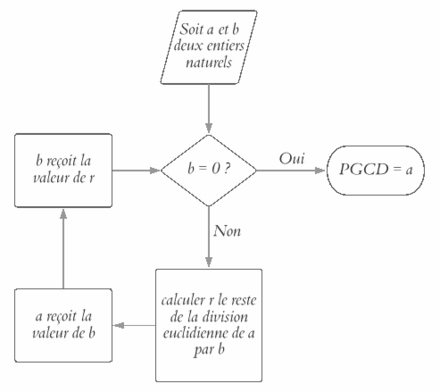
\includegraphics[scale=0.5]{algo.jpg}
    \caption{Algorithme Euclide}
    \label{fig:euclide}
\end{figure}

\end{definition}